\documentclass[a4paper,12pt]{article}

\usepackage[utf8x]{inputenc}
\usepackage[english]{babel}
\usepackage[margin=1in,includefoot]{geometry}

\usepackage{pgfplots}
\pgfplotsset{width=10cm,compat=1.12}
\usetikzlibrary{arrows}
\usepackage{amsmath}

\usepackage{indentfirst}
\usepackage{booktabs}

\usepackage[backref=false,pagebackref=true,citecolor=blue]{hyperref}
\hypersetup{colorlinks=true,urlcolor=blue,pdfborder={0 0 0}}

\setlength{\parindent}{2em}
\setlength{\parskip}{1em}

%\renewcommand{\arraystretch}{2}
%\renewcommand{\familydefault}{\sfdefault}

\usepackage{minted}
\renewcommand{\theFancyVerbLine}{\rmfamily\scriptsize\arabic{FancyVerbLine}}
\definecolor{whitesmoke}{rgb}{0.96,0.96,0.96}
\setminted{linenos,autogobble,breaklines,fontsize=\footnotesize,tabsize=4,numbersep=7pt,bgcolor=whitesmoke}
% \begin{minted}{cpp}
% \mintinline{cpp}{...}

\newcommand{\refspace}{\vspace{-2mm}}
\newcommand{\redarrow}{\textcolor{blue}{$\mathbf{\Rightarrow}$}}
\makeatletter
\def\BR@@bibitem#1#2\par{
	\let\backrefprint\BR@backrefprint
	\def\@linkcolor{black}
	\BRorg@bibitem{#1}#2\redarrow \thinspace \BR@backref{#1}
}
\makeatother

\author{Roland Bogosi}
\title{Market Prediction}

\begin{document}
\thispagestyle{empty}
	 
	\begin{center}
		\vspace{3.1in}
		
		{\sffamily\huge Market Prediction using Neural Networks}
		
		\vspace{0.4in}
		
		{\sffamily\LARGE Assignment Report}
		
		\vspace{0.3in}
		
		{\sffamily\Large January 4th, 2016}
		
		\vspace{3.2in}
	\end{center}
	
	\begin{flushright}
		{\sffamily\itshape\Large Roland Bogosi}
	\end{flushright}

\newpage
\thispagestyle{empty}
\section*{Table of Contents}

	\begingroup
	\renewcommand{\section}[2]{}
	\hypersetup{linkcolor=blue}
	\setlength{\parskip}{0em}
	\tableofcontents
	\endgroup

\newpage
\section{Introduction}

	The purpose of this classroom assignment is to use neural networks in order to predict stock market or currency fluctuations. There are many ways to tackle this time-series prediction problem, each of them having their own pros and cons:
	
	\textbf{Index Prediction} -- Try to teach the individual values of a series. This way the neural network will receive an input which in some form indicates the day we would like to evaluate it/predict for and as the output of the network, we get the prediction.
	
	\textbf{Indicator Prediction} -- Transform the dataset into indicators used during stock analysis, and teach the neural network the pattern of these. This way, the neural network will not be able to predict the index itself, but it should be able to predict the trend within the indicator that is used to make the actual decision if a stock should be purchased or not.
		
	In both cases, as described in \cite{op1997stock}, one of the main challenges was to decide what inputs and outputs should the neural network be trained for. My initial thought was to feed the date as input, and get the predicted index as the output. However, upon experimentation I learned that this model would not work, and after further researching, the winner method seemed to be having one or more input variables which are the index values of the previous days.

	\begin{figure}[!htbp]
		\centering
		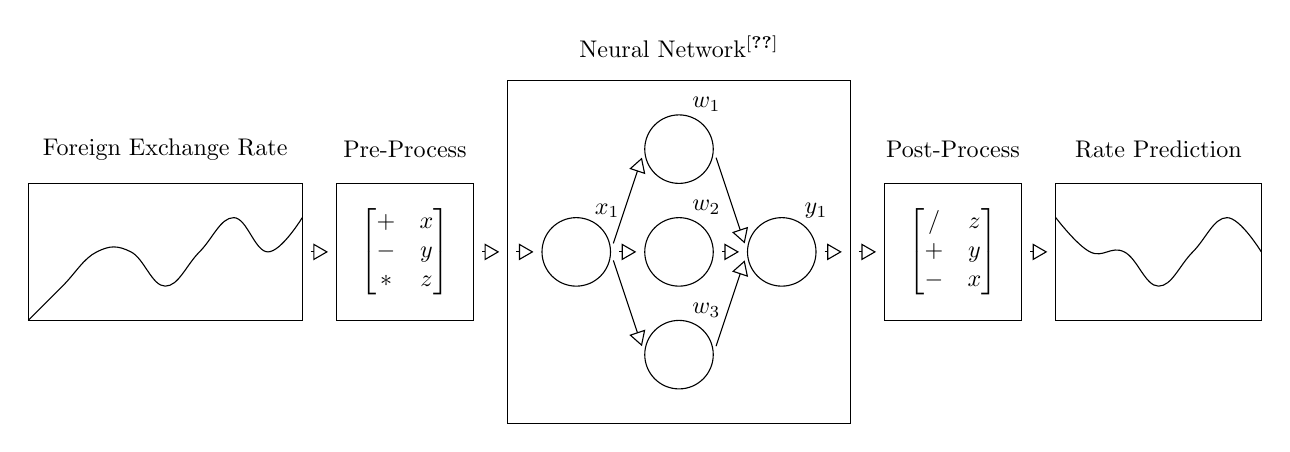
\begin{tikzpicture}[scale=0.87, transform shape]
		\tikzstyle{es} = [-open triangle 60]
		\draw [] (0,0) ellipse (0.5 and 0.5);
		\draw [] (0,1.5) ellipse (0.5 and 0.5);
		\draw [] (0,-1.5) ellipse (0.5 and 0.5);
		\draw [] (1.5,0) ellipse (0.5 and 0.5);
		\draw [] (-1.5,0) ellipse (0.5 and 0.5);
		\node (v1) at (-1,0) {};
		\node (v2) at (-0.5,1.5) {};
		\node (v3) at (-0.5,0) {};
		\node (v4) at (-0.5,-1.5) {};
		\node (v5) at (0.5,1.5) {};
		\node (v7) at (0.5,0) {};
		\node (v8) at (0.5,-1.5) {};
		\node (v6) at (1,0) {};
		\draw [es] (v1) edge (v2);
		\draw [es] (v1) edge (v3);
		\draw [es] (v1) edge (v4);
		\draw [es] (v5) edge (v6);
		\draw [es] (v7) edge (v6);
		\draw [es] (v8) edge (v6);
		\node (v9) at (-2.5,0) {};
		\node (v12) at (2.5,0) {};
		\node (v10) at (-2,0) {};
		\draw [es] (v9) edge (v10);
		\node (v11) at (2,0) {};
		\draw [es] (v11) edge (v12);
		\node at (0.4,2.15) {$w_1$};
		\node at (0.4,0.65) {$w_2$};
		\node at (0.4,-0.85) {$w_3$};
		\node at (2,0.6) {$y_1$};
		\node at (-1.05,0.6) {$x_1$};
		\node at (0,3) {Neural Network$^{[\ref{neurnet}]}$};
		\draw  (-2.5,2.5) rectangle (2.5,-2.5);
		\draw  (-5.5,-1) rectangle (-9.5,1);
		\draw  plot[smooth, tension=.7] coordinates {(-9.5,-1) (-9,-0.5) (-8.5,0) (-8,0) (-7.5,-0.5) (-7,0) (-6.5,0.5) (-6,0) (-5.5,0.5)};
		\node at (-7.5,1.5) {Foreign Exchange Rate};
		\node (v13) at (-5.5,0) {};
		\node at (-4,1.5) {Pre-Process};
		\draw [es] (-5,1) rectangle (-3,-1);
		\node (v14) at (-5,0) {};
		\node (v15) at (-3,0) {};
		\draw [es] (v13) edge (v14);
		\draw [es] (v15) edge (v9);
		\draw [es] (3,1) rectangle (5,-1);
		\node (v16) at (3,0) {};
		\node (v17) at (5,0) {};
		\node at (4,1.5) {Post-Process};
		\draw [es] (v12) edge (v16);
		\draw  (8.5,-1) rectangle (5.5,1);
		\draw  plot[smooth, tension=.7] coordinates {(5.5,0.5) (6,0) (6.5,0) (7,-0.5) (7.5,0) (8,0.5) (8.5,0)};
		\node at (7,1.5) {Rate Prediction};
		\node (v18) at (5.5,0) {};
		\draw [es] (v17) edge (v18);
		\node at (-4,0) {$ \begin{bmatrix}+ & x\\ - & y\\ * & z\end{bmatrix} $};
		\node at (4,0) {$ \begin{bmatrix}/ & z\\ + & y\\ - & x\end{bmatrix} $};
		\end{tikzpicture}
		\caption{Basic Architecture of the System}
		\label{sysarch}
	\end{figure}
	
	For the purposes of this classroom assignment, I decided focusing on using currency rates, since stock data has way too many outside factors influencing it. I would have had to analyze these outside factors for each stock individually and encode it as an input to the neural network in some form, in order to create an accurate model. For example, the stock of a car manufacturing company might go up when they hold a press release and announce a model, and might suddenly go down if the new model gets a bad review from a reputable source or an issue arises with it, possibly needing call-backs.

\newpage
\section{Network Structure}

	After examining existing papers in the field of stocks and neural networks, I came upon paper \cite{guresen2011using} which summarizes a multitude of previous experiments done in this topic, including the neural networks and training sets used with the varying degrees of success.

	\begin{figure}[!htbp]
		\centering
		\begin{tikzpicture}[x=1.5cm,y=1.5cm]
			\tikzstyle{es} = [-triangle 60]
			\draw [] (0,0) ellipse (0.5 and 0.5);
			\draw [] (0,1.5) ellipse (0.5 and 0.5);
			\draw [] (0,-1.5) ellipse (0.5 and 0.5);
			\draw [] (2.5,0) ellipse (0.5 and 0.5);
			\draw [] (-2.5,0) ellipse (0.5 and 0.5);
			\node (v1) at (-2,0) {};
			\node (v2) at (-0.5,1.5) {};
			\node (v3) at (-0.5,0) {};
			\node (v4) at (-0.5,-1.5) {};
			\node (v5) at (0.5,1.5) {};
			\node (v7) at (0.5,0) {};
			\node (v8) at (0.5,-1.5) {};
			\node (v6) at (2,0) {};
			\draw [es] (v1) edge (v2);
			\draw [es] (v1) edge (v3);
			\draw [es] (v1) edge (v4);
			\draw [es] (v5) edge (v6);
			\draw [es] (v7) edge (v6);
			\draw [es] (v8) edge (v6);
			\node (v9) at (-4.5,0) {};
			\node (v12) at (4.5,0) {};
			\node (v10) at (-3,0) {};
			\draw [es] (v9) edge (v10);
			\node (v11) at (3,0) {};
			\draw [es] (v11) edge (v12);
			\node at (-2.5,2.5) {\shortstack{Input\\layer}};
			\node at (0,2.5) {\shortstack{Hidden\\layers}};
			\node at (2.5,2.5) {\shortstack{Output\\layer}};
			\node at (0.5,2) {$w_1$};
			\node at (0.5,0.5) {$w_2$};
			\node at (0.5,-1) {$w_3$};
			\node at (3,0.5) {$y_1$};
			\node at (-2,0.5) {$x_1$};
		\end{tikzpicture}
		\caption{Structure of the Neural Network}
		\label{neurnet}
	\end{figure}

	The neural network shown in figure \ref{neurnet} is a multilayer perceptron network, whose purpose generally is to map a set of inputs onto a set of outputs, as such its application is popular for solving time-series prediction problems. It has a single input, $x_1$, which is the index of the stock or currency for that day. The output of the network, $y_1$, is the predicted value for the \textit{next} day.
	
	The number of hidden layers in the network varies based on how many training samples (days) we would like to train the network on, and also on how many days we would like to predict beyond the training samples. While the general rule is to have $x_n \cdot 2$ hidden layers, I evaluated this during several trial and error runs and it did not seem to work well with this application. Even with the momentum learning parameter ($m$) set to a high value, $0.9 < m < 1$, the neural network was not able to accurately fit the data, it only generated an approximate oscillation.
	
	The neural network is trained with backpropagation, which is a supervised learning method. The network weights are randomly initialized to values between the range of $[0.25..0.35]$, which was determined to yield the best results after a few trial and error runs. The activation function used with the trainer is sigmoid: $f(x) = \frac{1}{e^{-\alpha \cdot x} + 1}$
	
	After some experimentation, I found the number of hidden layers in order to accurately fit the data as a result of $1,000$ iterations of the backpropagation teacher algorithm, to be an approximation of the size of training samples. As such, the network configuration will vary for each experiment individually.

\section{Experiments}
\subsection{Error Calculation}

	I conducted a multitude of experiments in order to try and find a configuration with the lowest learning and prediction error for each common training size and prediction requirement. In order to quantify the error, I had to look up the methods available for determining the accuracy of trend estimation and found a comparison between the common methods in paper \cite{armstrong1992error}.
	
	\textit{MAPE} (\textit{Mean Absolute Percentage Error}) ended up as being the winning method, since it has been used in many other papers, such as \cite{majhi2009efficient}, which allows me to have a baseline comparison for my results. \textit{MAPE} is defined as:\\
	$$ \epsilon = (\frac{1}{n} \sum_{i=1}^{n} \frac{x_i - x_i'}{x_i}) \cdot 100 \label{mape} $$\\
	where $n$ is the number of predictions, $x_i$ is the actual value, and $x_i'$ is the predicted value.
	
\subsection{Case Study: 7-day prediction for 30-day EUR/USD data}
	
	In this experiment, I focused my efforts on tuning a neural network to predict as accurately as possible a full week's exchange rates in advance for the currency pair EUR/USD.
	
	In order to do this, I set up a script to find the best possible parameters for the given dataset by training and evaluating neural networks with varying parameters using the \mintinline{csharp}{MarketPrediction.NeuralNetwork.TrainAndEval()} API. A snippet of this script can be observed in listing \ref{bruteforce}.
	
	\begin{listing}[!htbp]
		\begin{minted}{csharp}
double smallestError = double.MaxValue;

for (int inputLayers = 1; inputLayers < min(10, dataSetSize); inputLayers++) {
	for (int hiddenLayers = 1; hiddenLayers < dataSetSize; hiddenLayers++) {
		// ...additional parameters as needed...
		
		double error = TrainAndEval(inputLayers, hiddenLayers, ...);
		
		if (error < smallestError) {
			// save current parameters as best-performing...
			smallestError = error;
		}
	}
}
		\end{minted}
		\caption{Exhaustive Search for Highest Accuracy}
		\label{bruteforce}
	\end{listing}
	
	Since the aforementioned script can be easily parallelized by asynchronously running one or more of the loops, it is a fast and easy method to find the best configuration for any data set. The error value the search is optimizing for is the equation described in section \ref{mape}.
	
	\begin{figure}[!htbp]
		\centering
		\begin{tikzpicture}
		\begin{axis}[
			xlabel={Days},
			ylabel={Index},
			legend pos=north west,
			ymajorgrids=true,
			grid style=dashed,
			legend entries={Actual Rates,Estimate,Prediction}
		]
			\addplot[blue,mark=*]  table {eur_usd_august_30.txt};
			\addplot[red,mark=*]   table {eur_usd_august_30_neuron.txt};
			\addplot[green,mark=*] table {eur_usd_august_30_neuron_pred.txt};
		\end{axis}
		\end{tikzpicture}
		\caption{EUR/USD Rates for August 2015}
		\label{eur_usd_august_30_neuron}
	\end{figure}
	
	The network shown in figure \ref{eur_usd_august_30_neuron} was trained for $1,000$ iterations, with a \textit{learning rate} of $0.05$ and a \textit{momentum learning coefficient} of $0.988$. It has $1$ input and $30$ hidden layers.
	
	Its mean absolute percentage error for the training set is $0.2682\%$, while the prediction error for the next 7 days is $0.7129\%$.
	
	\begin{figure}[!htbp]
		\centering
		\begin{tikzpicture}
		\begin{axis}[
			xlabel={Days},
			ylabel={Index},
			legend pos=north west,
			ymajorgrids=true,
			grid style=dashed,
			legend entries={Actual Rates,Estimate,Prediction}
		]
			\addplot[blue,mark=*]  table {eur_usd_august_30.txt};
			\addplot[red,mark=*]   table {eur_usd_august_30_genetic.txt};
			\addplot[green,mark=*] table {eur_usd_august_30_genetic_pred.txt};
		\end{axis}
		\end{tikzpicture}
		\caption{EUR/USD Rates for August 2015}
		\label{eur_usd_august_30_genetic}
	\end{figure}
	
	As a comparison, in figure \ref{eur_usd_august_30_genetic}, the same dataset is taught with a genetic algorithm. The algorithm ran for $1,000$ iterations, while having a population size of $100$ and using a selection method which selects the chromosomes with the highest fitness value. The configuration had 1 variable input and 3 constants, as explained in table \ref{geninput}.
	
	The output of the genetic algorithm, meaning the fittest chromosome, after $1,000$ iterations is the following equation:\\
	$$ (b \cdot \frac{b \cdot \frac{c}{b}}{\frac{c \cdot b}{b}}) \cdot \frac{a}{(b \cdot c) \cdot \frac{\frac{c}{d}}{b}} $$\\
	which can be simplified to:\\
	$$ \frac{a \cdot b \cdot c}{2} $$\\
	where variables are as shown in table \ref{geninput}.
		
	\begin{table}[!htbp]
		\centering
		\begin{tabular}{@{}rcl@{}}
			\toprule
			\multicolumn{1}{c}{\textbf{\$}} & \textbf{Value} & \multicolumn{1}{c}{\textbf{Explanation}} \\ \midrule
			a & $1.0875$ & variable input 1: index value of current day \\
			b & $1.0830$ & minimum of training set \\
			c & $1.0977$ & arithmetic average of training set \\
			d & $1.1143$ & maximum of training set \\ \bottomrule
		\end{tabular}
		\caption{Genetic Algorithm Inputs: Variables and Constants}
		\label{geninput}
	\end{table}
		
	The final fittest chromosome has a mean absolute percentage error of $0.2507\%$ against the training set, and a prediction error of $0.6872\%$ for the next 7 days.
	
\newpage
\section{Bibliography}

	\begingroup
	\renewcommand{\section}[2]{}
		\bibliography{report} 
		\bibliographystyle{ieeetr}
	\endgroup

\end{document}